%
% auth: Mattijs Korpershoek
% mail: <mattijs.korpershoek@gmail.com>
%

\section{Context}

\subsection{Company}
\begin{frame}
    \frametitle{Company}
    \begin{minipage}{0.49\textwidth}
        \begin{itemize}
            \item Hired by Celad
            \item Worked at Intel which is one of Celad's client
            \item CPU manufacturer, why Android?
            \item Android smartphones and tablets with Intel inside
            \item Contributions on HAL
        \end{itemize}
    \end{minipage}
    \begin{minipage}{0.49\textwidth}
        \flushright
        
\includegraphics[height=1cm]{../../report/src/img/logocelad.jpg} \hspace{0.2cm}
        
\includegraphics[height=1cm]{../../report/src/img/logointel.jpg} \\[0.5cm]
        
\includegraphics[height=1cm]{./img/androidLogo.png} \\
        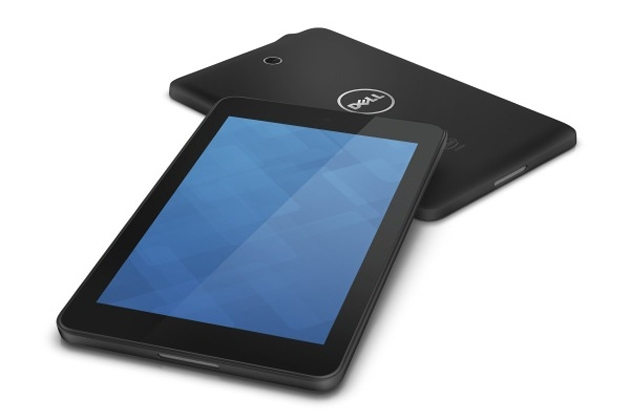
\includegraphics[height=0.4\textheight]{./img/dell-venue.jpg}
    \end{minipage}
\end{frame}

\subsection{HAL}
\begin{frame}
    \frametitle{Hardware Abstraction Layer (HAL)}
    \begin{itemize}
        \item Link between kernel and applications
        \item Vendor specific implementation
        \item Difficult to deal with all the hardware variations
        \item Each vendor solves the same problem in their own way
    \end{itemize}
\end{frame}

\subsection{Parameter-framework}
\begin{frame}
    \frametitle{Parameter-framework}
    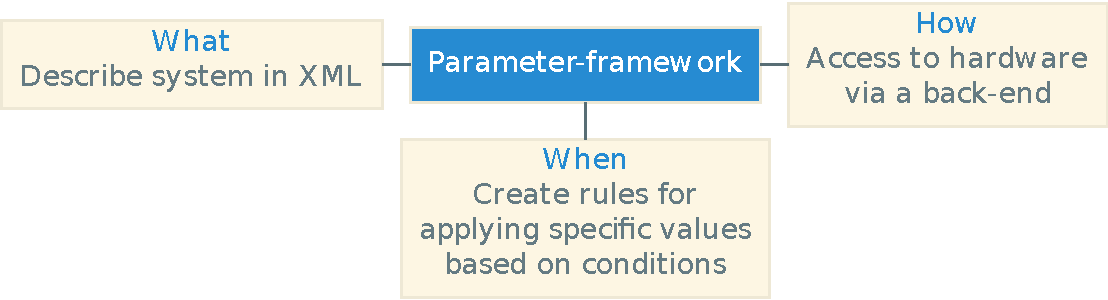
\includegraphics[width=\textwidth]{./img/pfwContext.pdf}
    \begin{block}{Why open-source it?}
        \begin{itemize}
            \item Give the component some visibility
            \item Make it an Android standard
        \end{itemize}
    \end{block}
\end{frame}
